\documentclass[10pt]{beamer}

%%%
% PREAMBLE FOR THIS DOC 
%%%
%https://tex.stackexchange.com/questions/68821/is-it-possible-to-create-a-latex-preamble-header
\usepackage{/Users/miw267/Repos/csci246_spring2025/slides/preambles/beamer_preamble_for_CSCI246}

\usetikzlibrary{matrix}


%%% TRY TO RESHOW TOC AT EACH SECTION START (with current section highlighted)
% Reference: https://tex.stackexchange.com/questions/280436/how-to-highlight-a-specific-section-in-beamer-toc
\newcommand\tocforsect[2]{%
  \begingroup
  \edef\safesection{\thesection}
  \setcounter{section}{#1}
  \tableofcontents[#2,currentsection]
  \setcounter{section}{\safesection}
  \endgroup
}


%%%% HERES HOW TO DO IT CORRECTLY
% FIRST IN .STY FILE, DO
%\usetheme[sectionpage=none]{metropolis}
% THEN AT EACH SECTION DO
%\begin{frame}{Outline}
%  \tableofcontents[currentsection]	
%\end{frame}



%\setbeamertemplate{navigation symbols}{}
%\setbeamertemplate{footline}[frame number]{}


%%%
% DOCUMENT
%%%

\begin{document}

%\maketitle

%% Title page frame
%\begin{frame}
%    \titlepage 
%\end{frame}





\title{03/07/2025: Catch-Up Day}
\author{CSCI 246: Discrete Structures}
\date{Textbook reference: None}

\begin{frame}
    \titlepage 
\end{frame}


\begin{frame}
\footnotesize 
\begin{mygreenbox}[title=Graded Quiz Pickup]
Quizzes are in the front of the room, grouped into four bins (A-G, H-L, M-R, S-Z) by last name. The quizzes are upside down with your last name on the back. Come find yours before, during, or after class.  Only turn the quiz over if it's yours.
\end{mygreenbox} 
\vfill 

%\begin{myredbox}[title=Announcement: How to be sure you're reading the right section]
%\begin{enumerate}
%	\item Check the current version of the syllabus to confirm the reading for the \textbf{next} course meeting sometime during (or after) class.  
%	\item The most current version of the syllabus can always be found at the \href{https://github.com/mikewojnowicz/csci246_spring2025}{course repo}.  
%\end{enumerate}
%\end{myredbox}

\vfill 


\begin{myyellowbox}[title=Today's Agenda]
\begin{itemize}
	\item Problems quiz (15 mins)
	\item Course feedback ($\approx$ 10 mins)
%	%
%	\begin{itemize}
%	\footnotesize 
%	\item Review induction 
%	\end{itemize}
%	%
	\item Group exercises ($\approx$ 20 mins)
\end{itemize}

%	Rationale for group exercises: we got shortchanged on time last couple days, and I already did a lot of lectures, so I want you to practice. Next problems quiz will cover relations and functions: Hamkins and 
%	
\end{myyellowbox}
\vfill 

\end{frame}

\begin{frame}[standout]
Feedback on Wednesday's Quiz 
\end{frame}



\begin{frame}{Scores On Reading Quiz (Binomial Coefficients)}
\footnotesize 
\begin{figure}[ht]
        \centering
        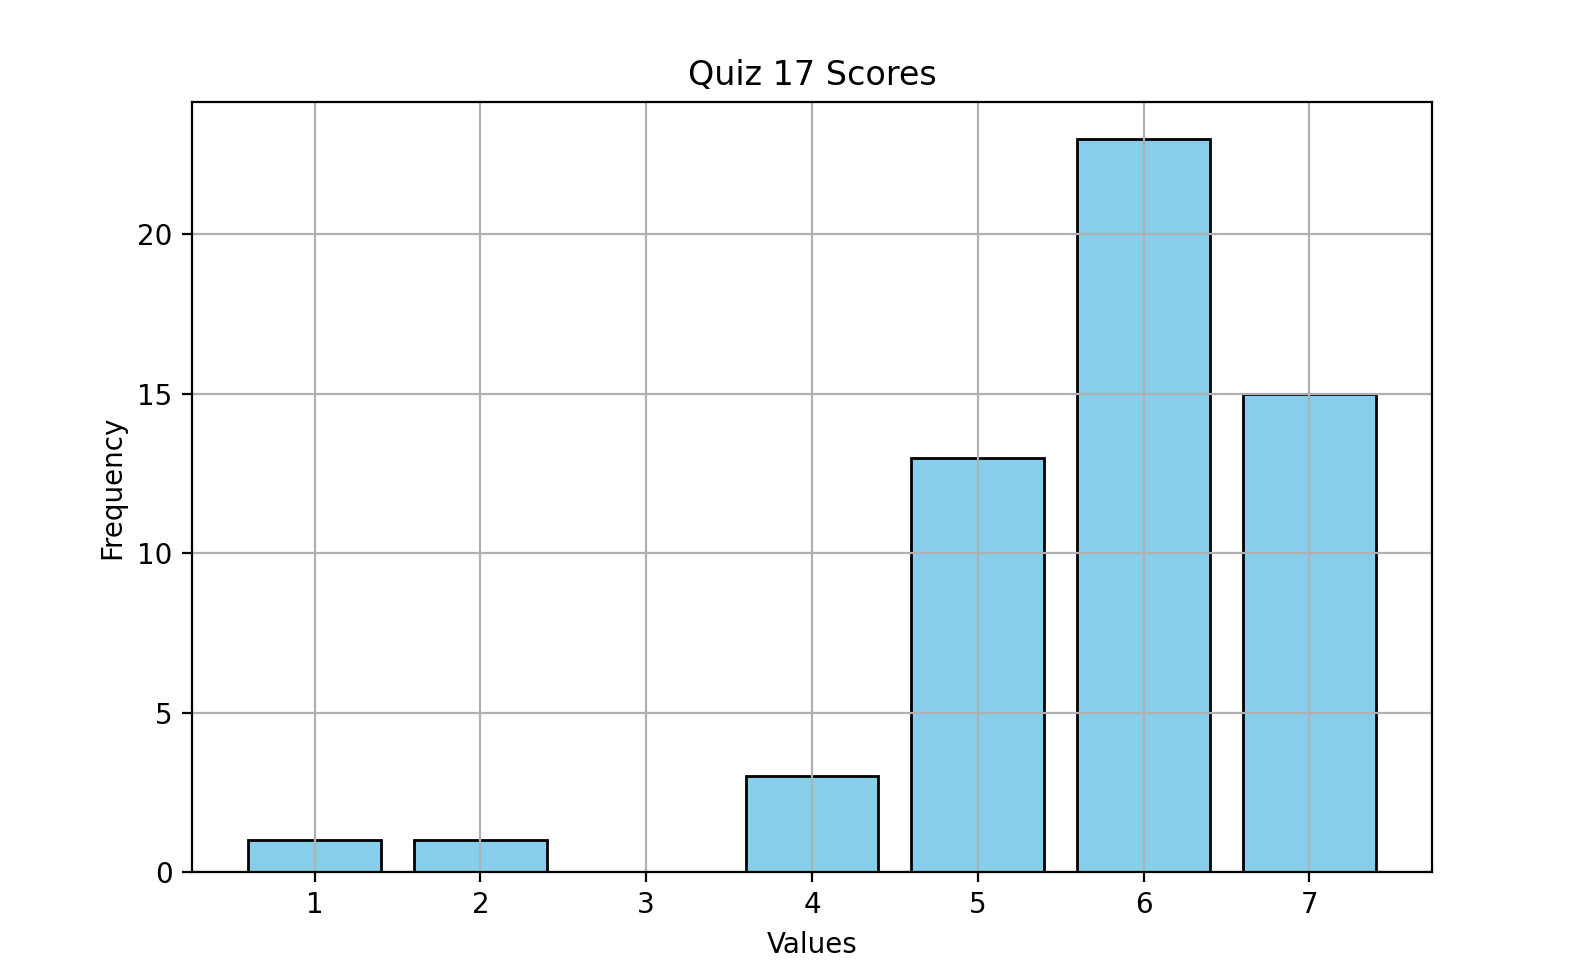
\includegraphics[width=.8\textwidth]{images/reading_quiz_scores}
   		 \caption{Median Score = 6/6 (100\%)}
\end{figure}
%\vfill 
%\textbf{Rubric.}  	
%\begin{itemize}
%\item  5 points for correctly answering that the relation WAS a function.
%\item 5 points for correct explanation.
%\item 1 point EC for additional correct explanation.
%\end{itemize}
\end{frame}

\begin{frame}{Counting Lattice Paths}
\footnotesize 
\begin{mygreenbox}[title= \text{Original Problem}]
%
\begin{columns}
\begin{column}{.4\textwidth}
 Suppose we want to count the number of grid paths from the lower left corner to the upper right corner in which each step of the path either goes one unit to the right or one unit vertically. How many paths are there?
\end{column}
\hfill 
\begin{column}{.4\textwidth}
\begin{center}
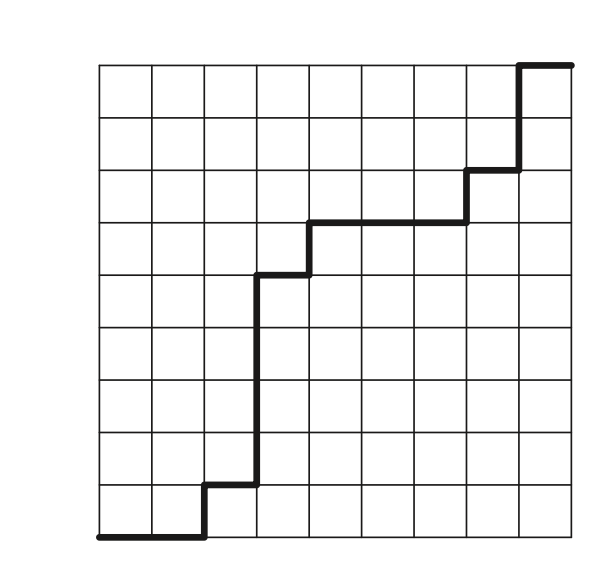
\includegraphics[width=.7\textwidth]{images/lattice_paths.png}
\end{center}	
\end{column}
\end{columns}


%
\end{mygreenbox}

\vfill 
\begin{myyellowbox}[title= \text{Erik's Problem}] How many paths would there be if the paths were allowed go  down and backwards, but not cross itself?	
\end{myyellowbox}
\vfill 
\begin{myredbox}[title= \text{Status}] This is still open!  I asked one of the smartest people I know, and he said:\\ 

\enquote{I feel like you are trying to nerd snipe me right now while Emily wants me to do chores.}  Later:  \enquote{I’m unsure of an answer but this is a fun problem.} 
\end{myredbox}

\end{frame}

\begin{frame}[standout]
Problems Quiz
\end{frame}

\begin{frame}

\begin{mygreenbox}[title= \text{Problems Quiz (Equivalence Relations, Partitions, and Functions)}]
\footnotesize 
\begin{enumerate}\footnotesize 
     \item  Let $A =\set{1,2,3,4}$ and $B=\set{5,6,7}$.  Let $f$ be the relation
	\[  f=\set{(?,?), (2,6),(3,6), (4,7)}\]
	Find replacements for (?,?) so that each of the following is true.
	\begin{itemize} \footnotesize 
		\item [a.] The relation $f$ is not a function from $A$ to $B$.
		\item [b.] The relation $f$ is a function from $A$ to $B$ but is not onto $B$.
		\item [c.] The relation $f$ is a function from $A$ to $B$ and is onto $B$.
	\end{itemize}
	\item Fourteen people join hands for  dance.  Suppose seven of these people are men, and the other seven are women.
	\begin{itemize}\footnotesize 
	\item [a.]  In how many different ways can they join hands for a circle dance, assuming they alternate in gender around the circle?
	\item [b.] How many different ways can they join hands for a line dance, assuming they alternate in gender along the line?
	\end{itemize}
	\item Prove Proposition 15.11:  Let $R$ be an equivalence relation on the set $A$ and let $a,x,y \in A$. If $x,y \in [a]$, then $xRy$.
	\end{enumerate}
\end{mygreenbox}
	
\end{frame}


\begin{frame}[standout]
Course Feedback
\end{frame}

\begin{frame}

\begin{myyellowbox}[title= \text{Course Feedback Instructions}]
Please write your name on a piece of paper and answer the questions below. 
\end{myyellowbox}

\vfill 
\begin{mygreenbox}[title= \text{Course Feedback}]
\begin{enumerate}
	\item What aspects of the course so far are you enjoying?
	\item What aspects of the course so far are you \textbf{not} enjoying? 
	\item What aspects of the course so far are helping with your learning?
	\item What aspects of the course so far are hindering your learning?
	\item What other comments would you like to make about the course so far (e.g. proposed tweaks)? 
\end{enumerate}
\end{mygreenbox}

	
\end{frame}






\begin{frame}[standout]
Group exercises (Binomial Coefficients)
\end{frame}


\end{document}
